\chapter{Изменение скалярного поля  для дивергентного поля скоростей}
\label{app:div_df}

\begin{figure}[h]
	\centering
	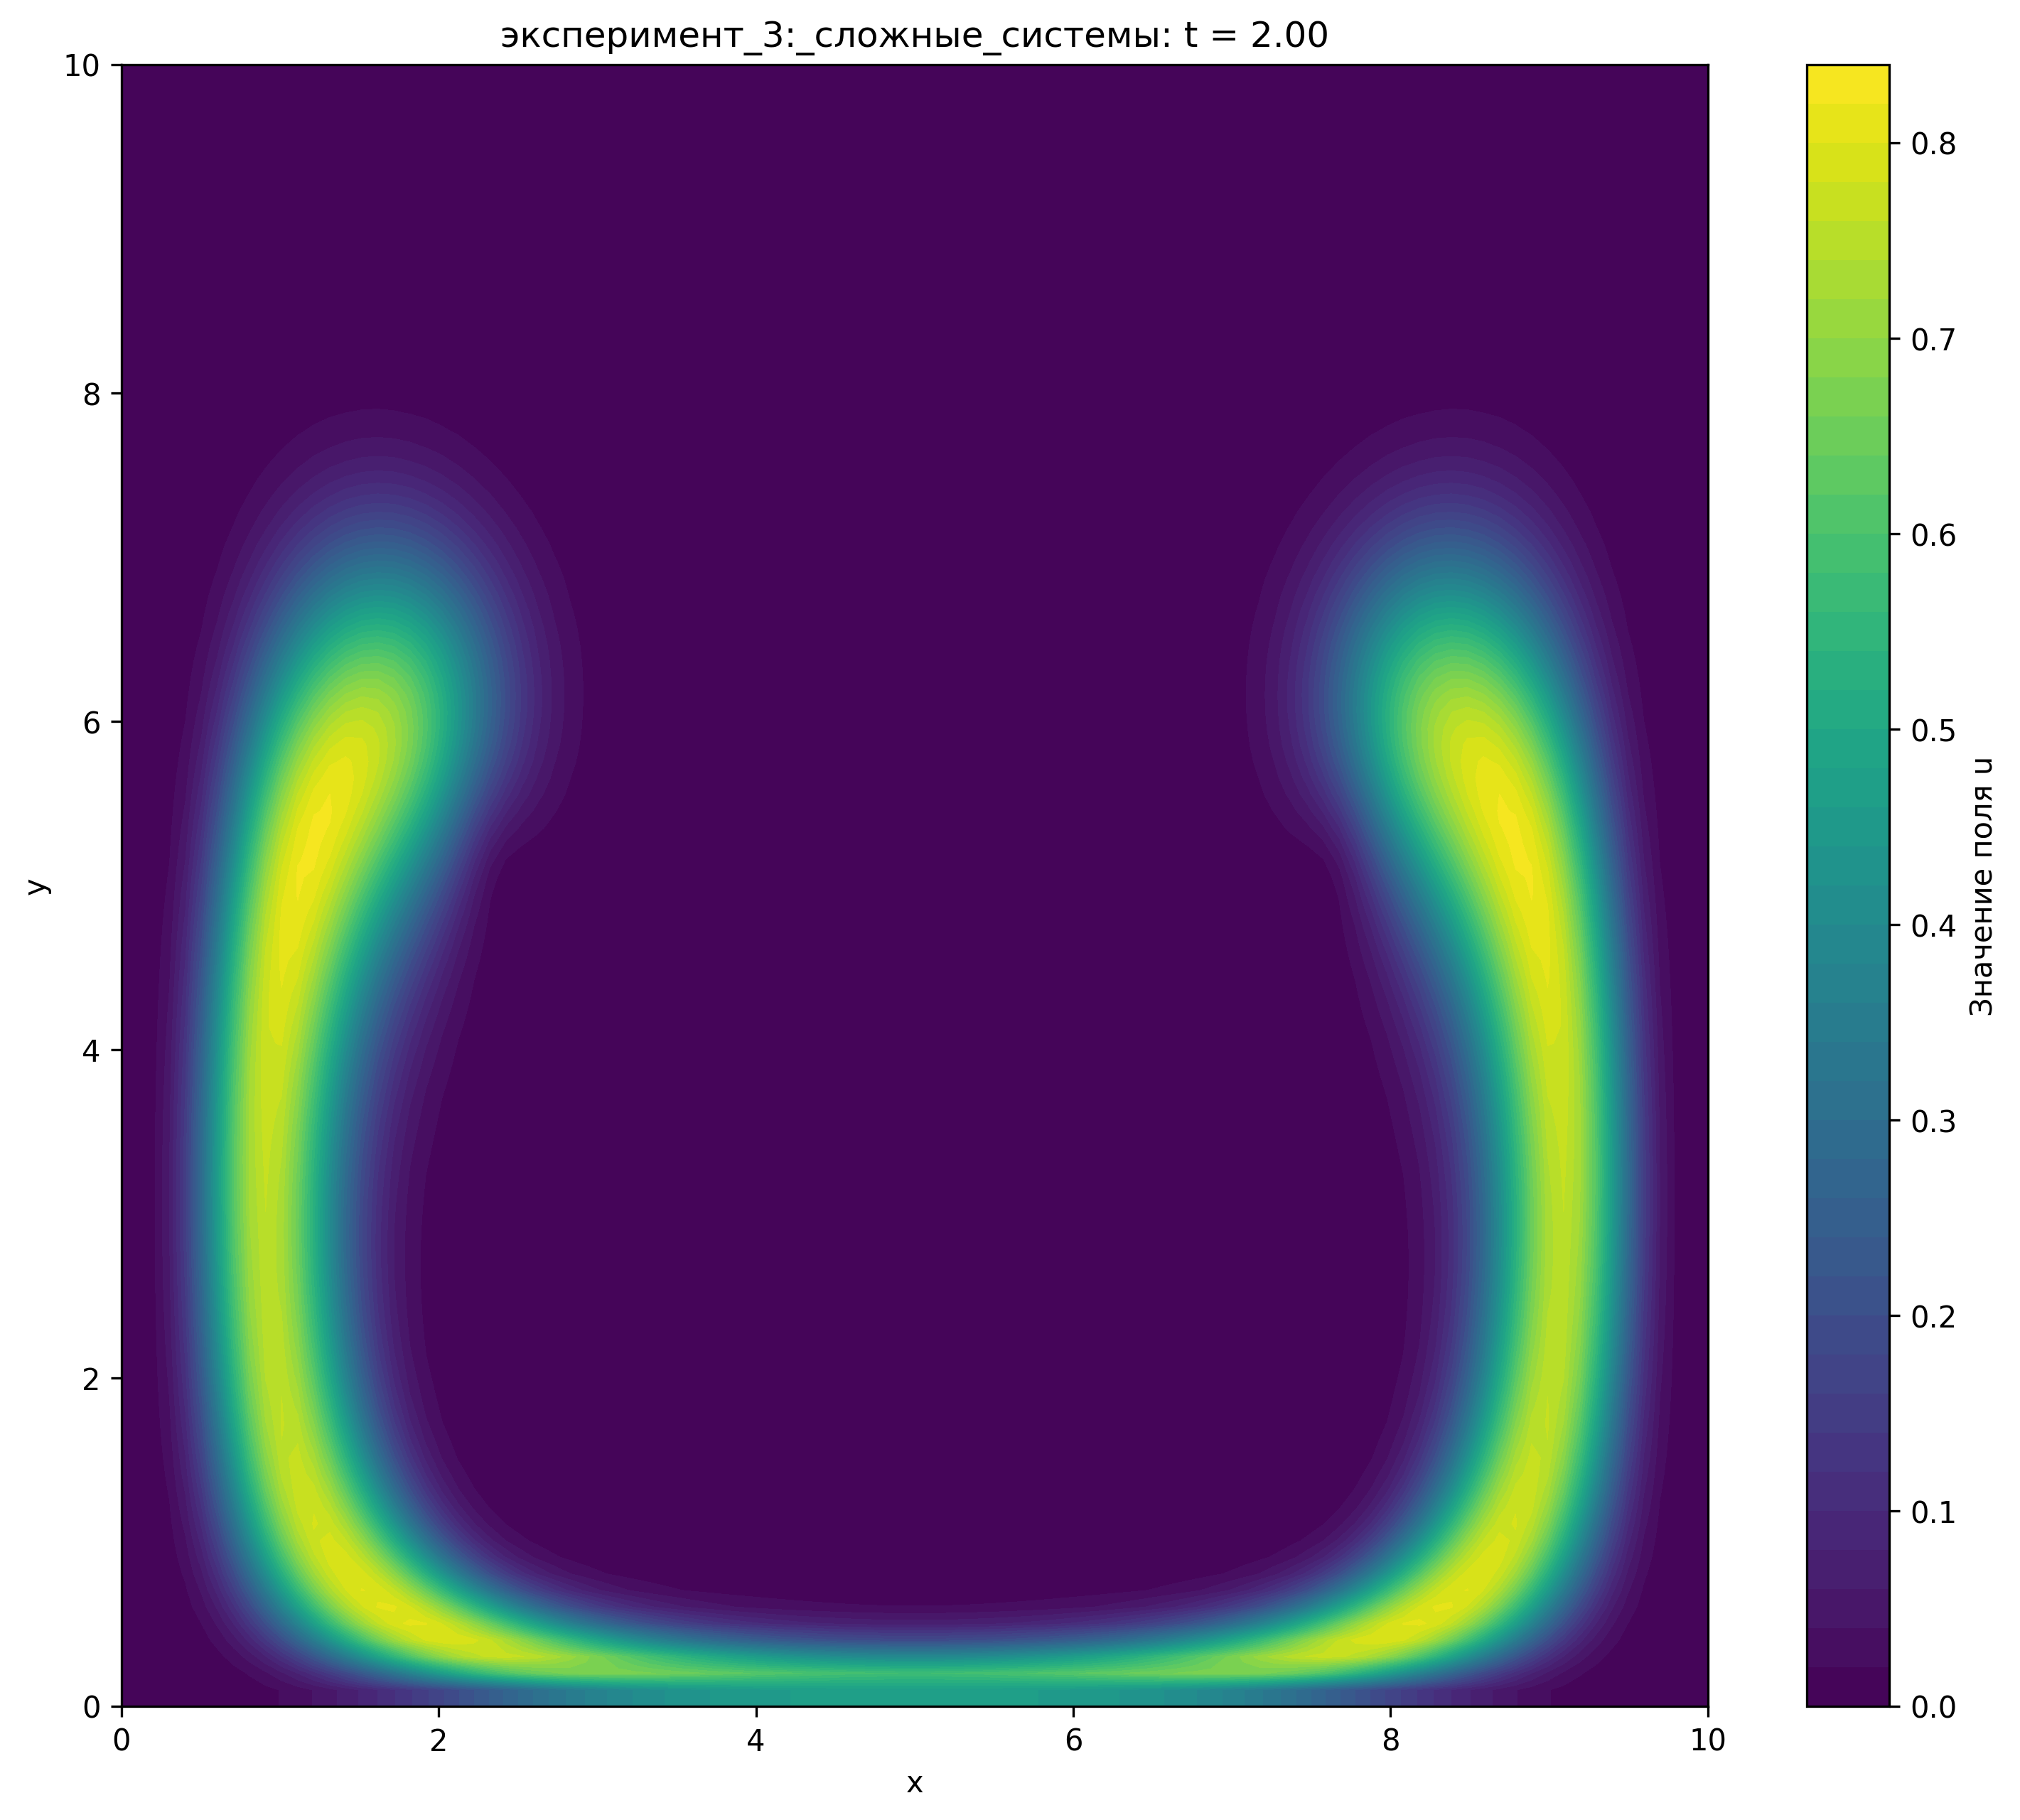
\includegraphics[width=0.6\textwidth]{imgs/эксперимент_3:_сложные_системы_t2.00.png}
	\caption{Скалярное поле в момент времени $t=2$ }
\end{figure}
\begin{figure}[h]
	\centering
	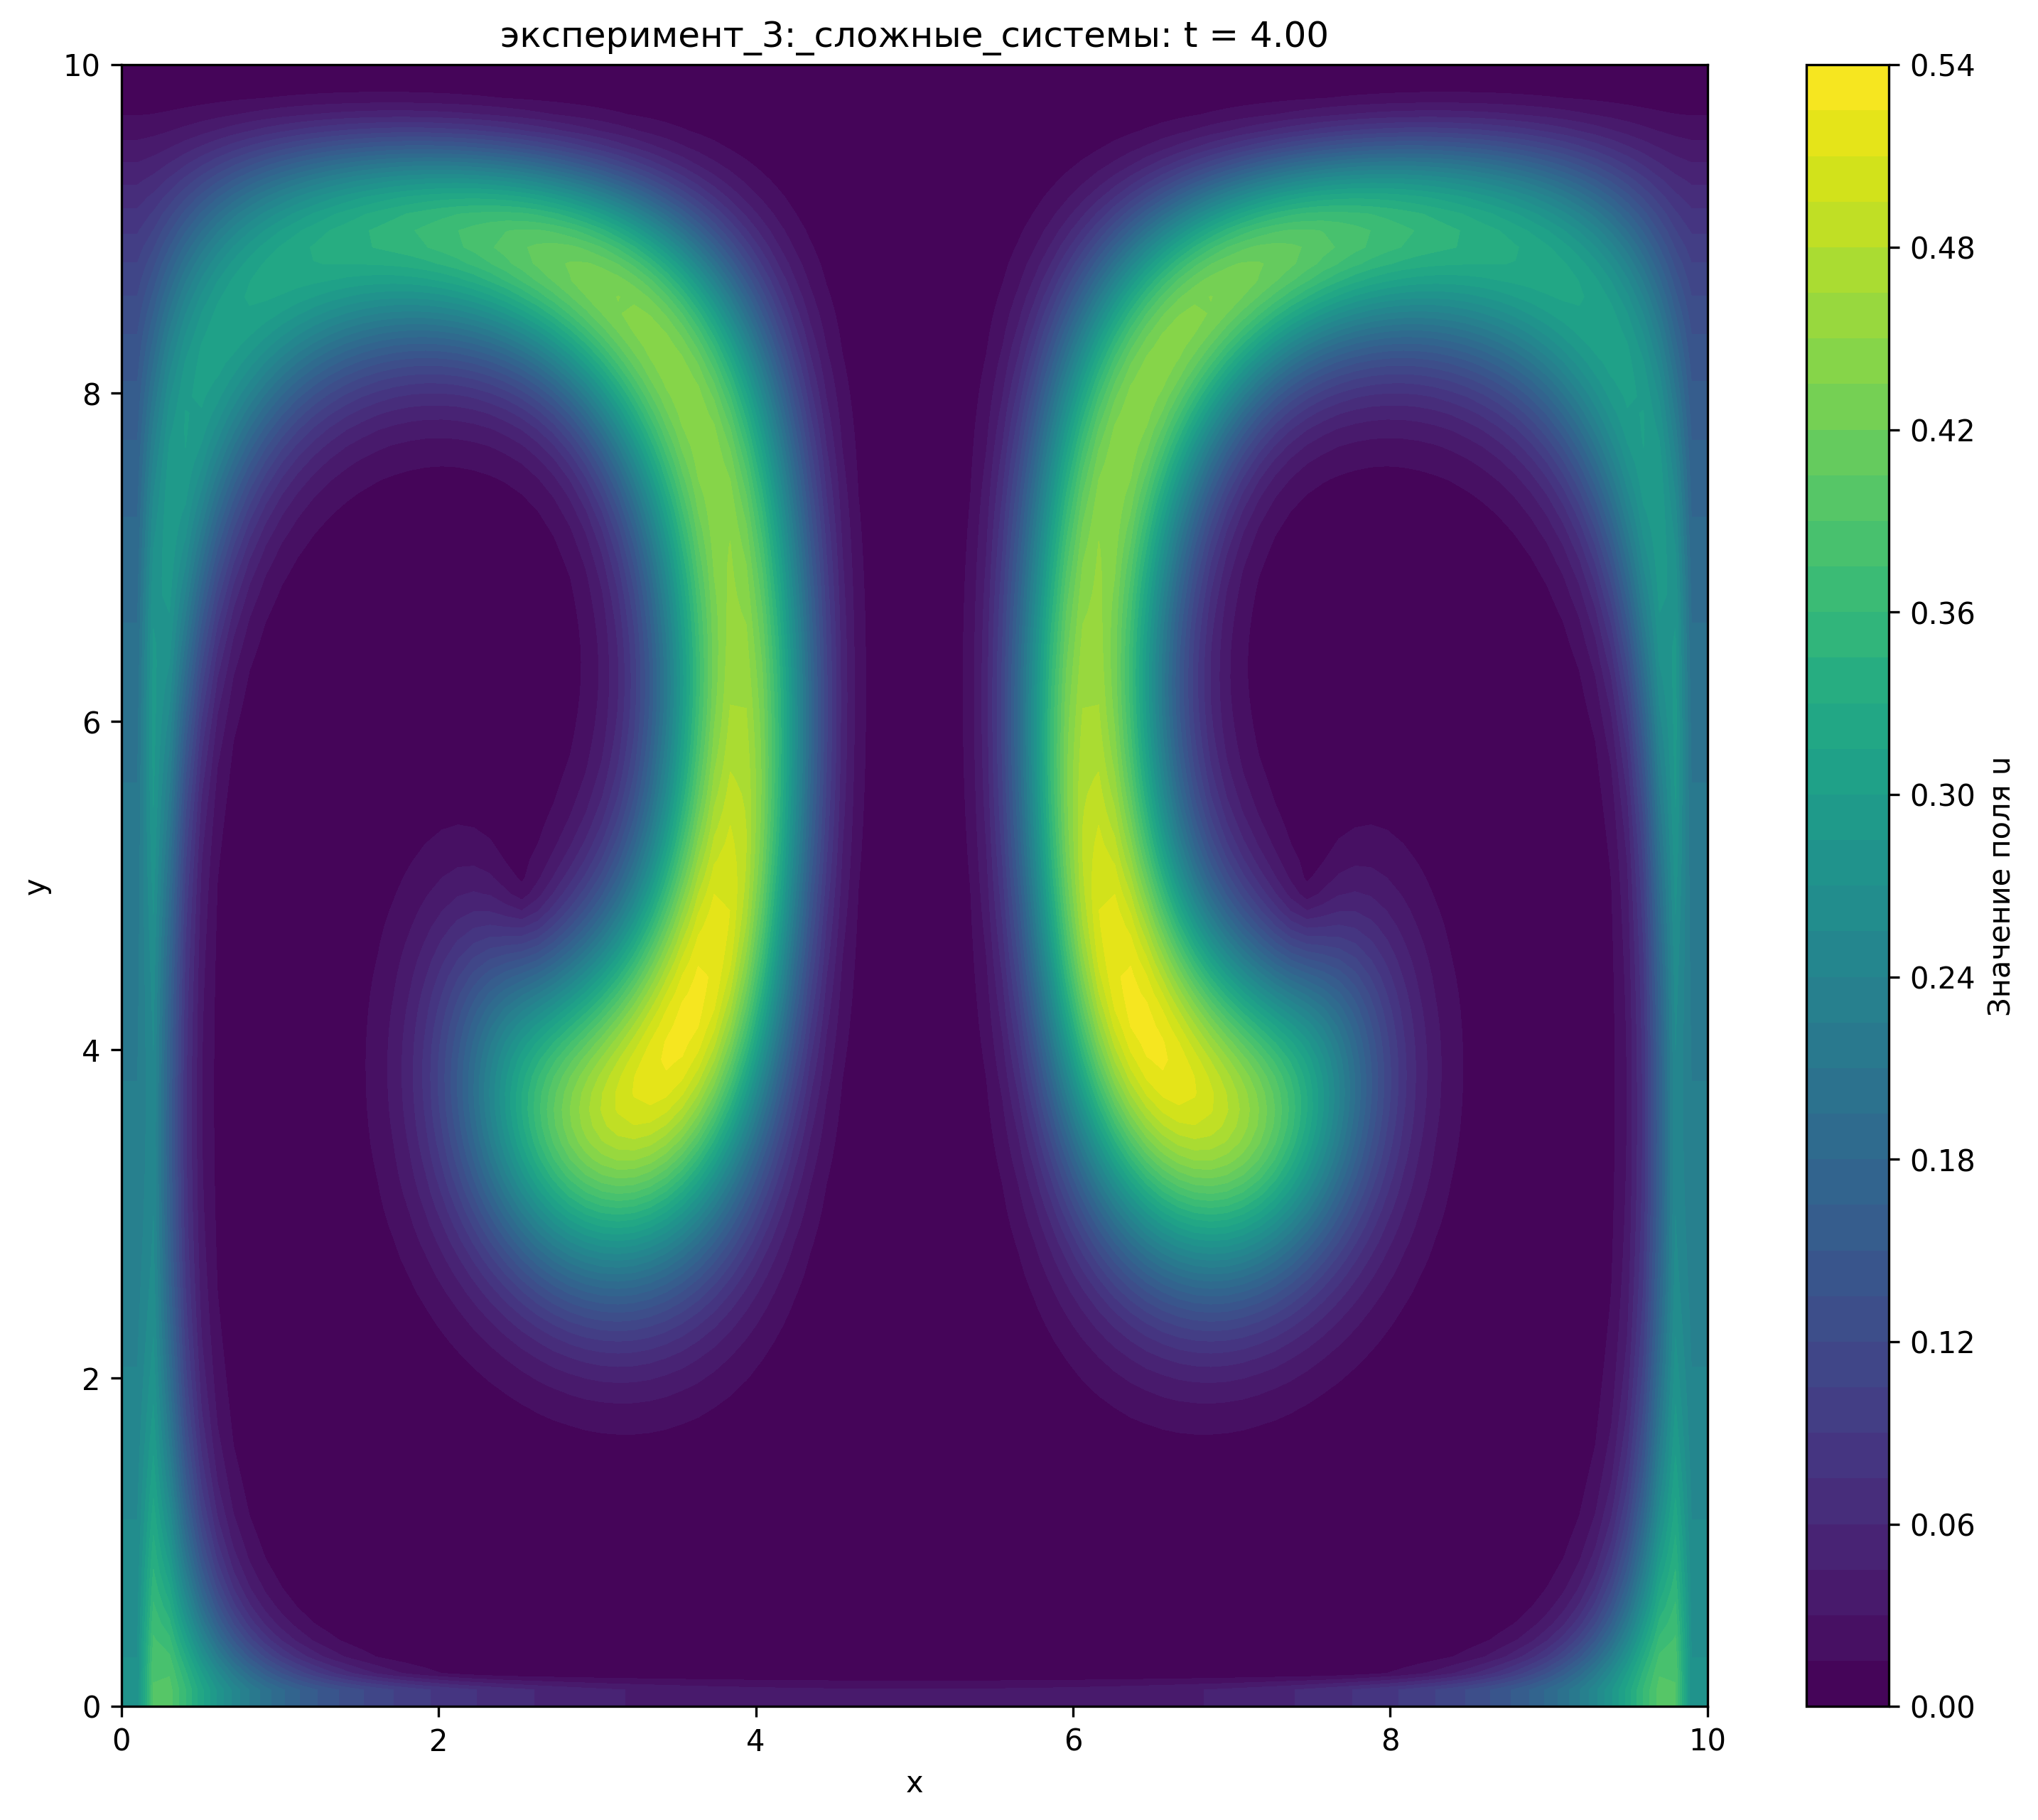
\includegraphics[width=0.6\textwidth]{imgs/эксперимент_3:_сложные_системы_t4.00.png}
	\caption{Скалярное поле в момент времени $t=4$}
\end{figure}
\begin{figure}[h]
	\centering
	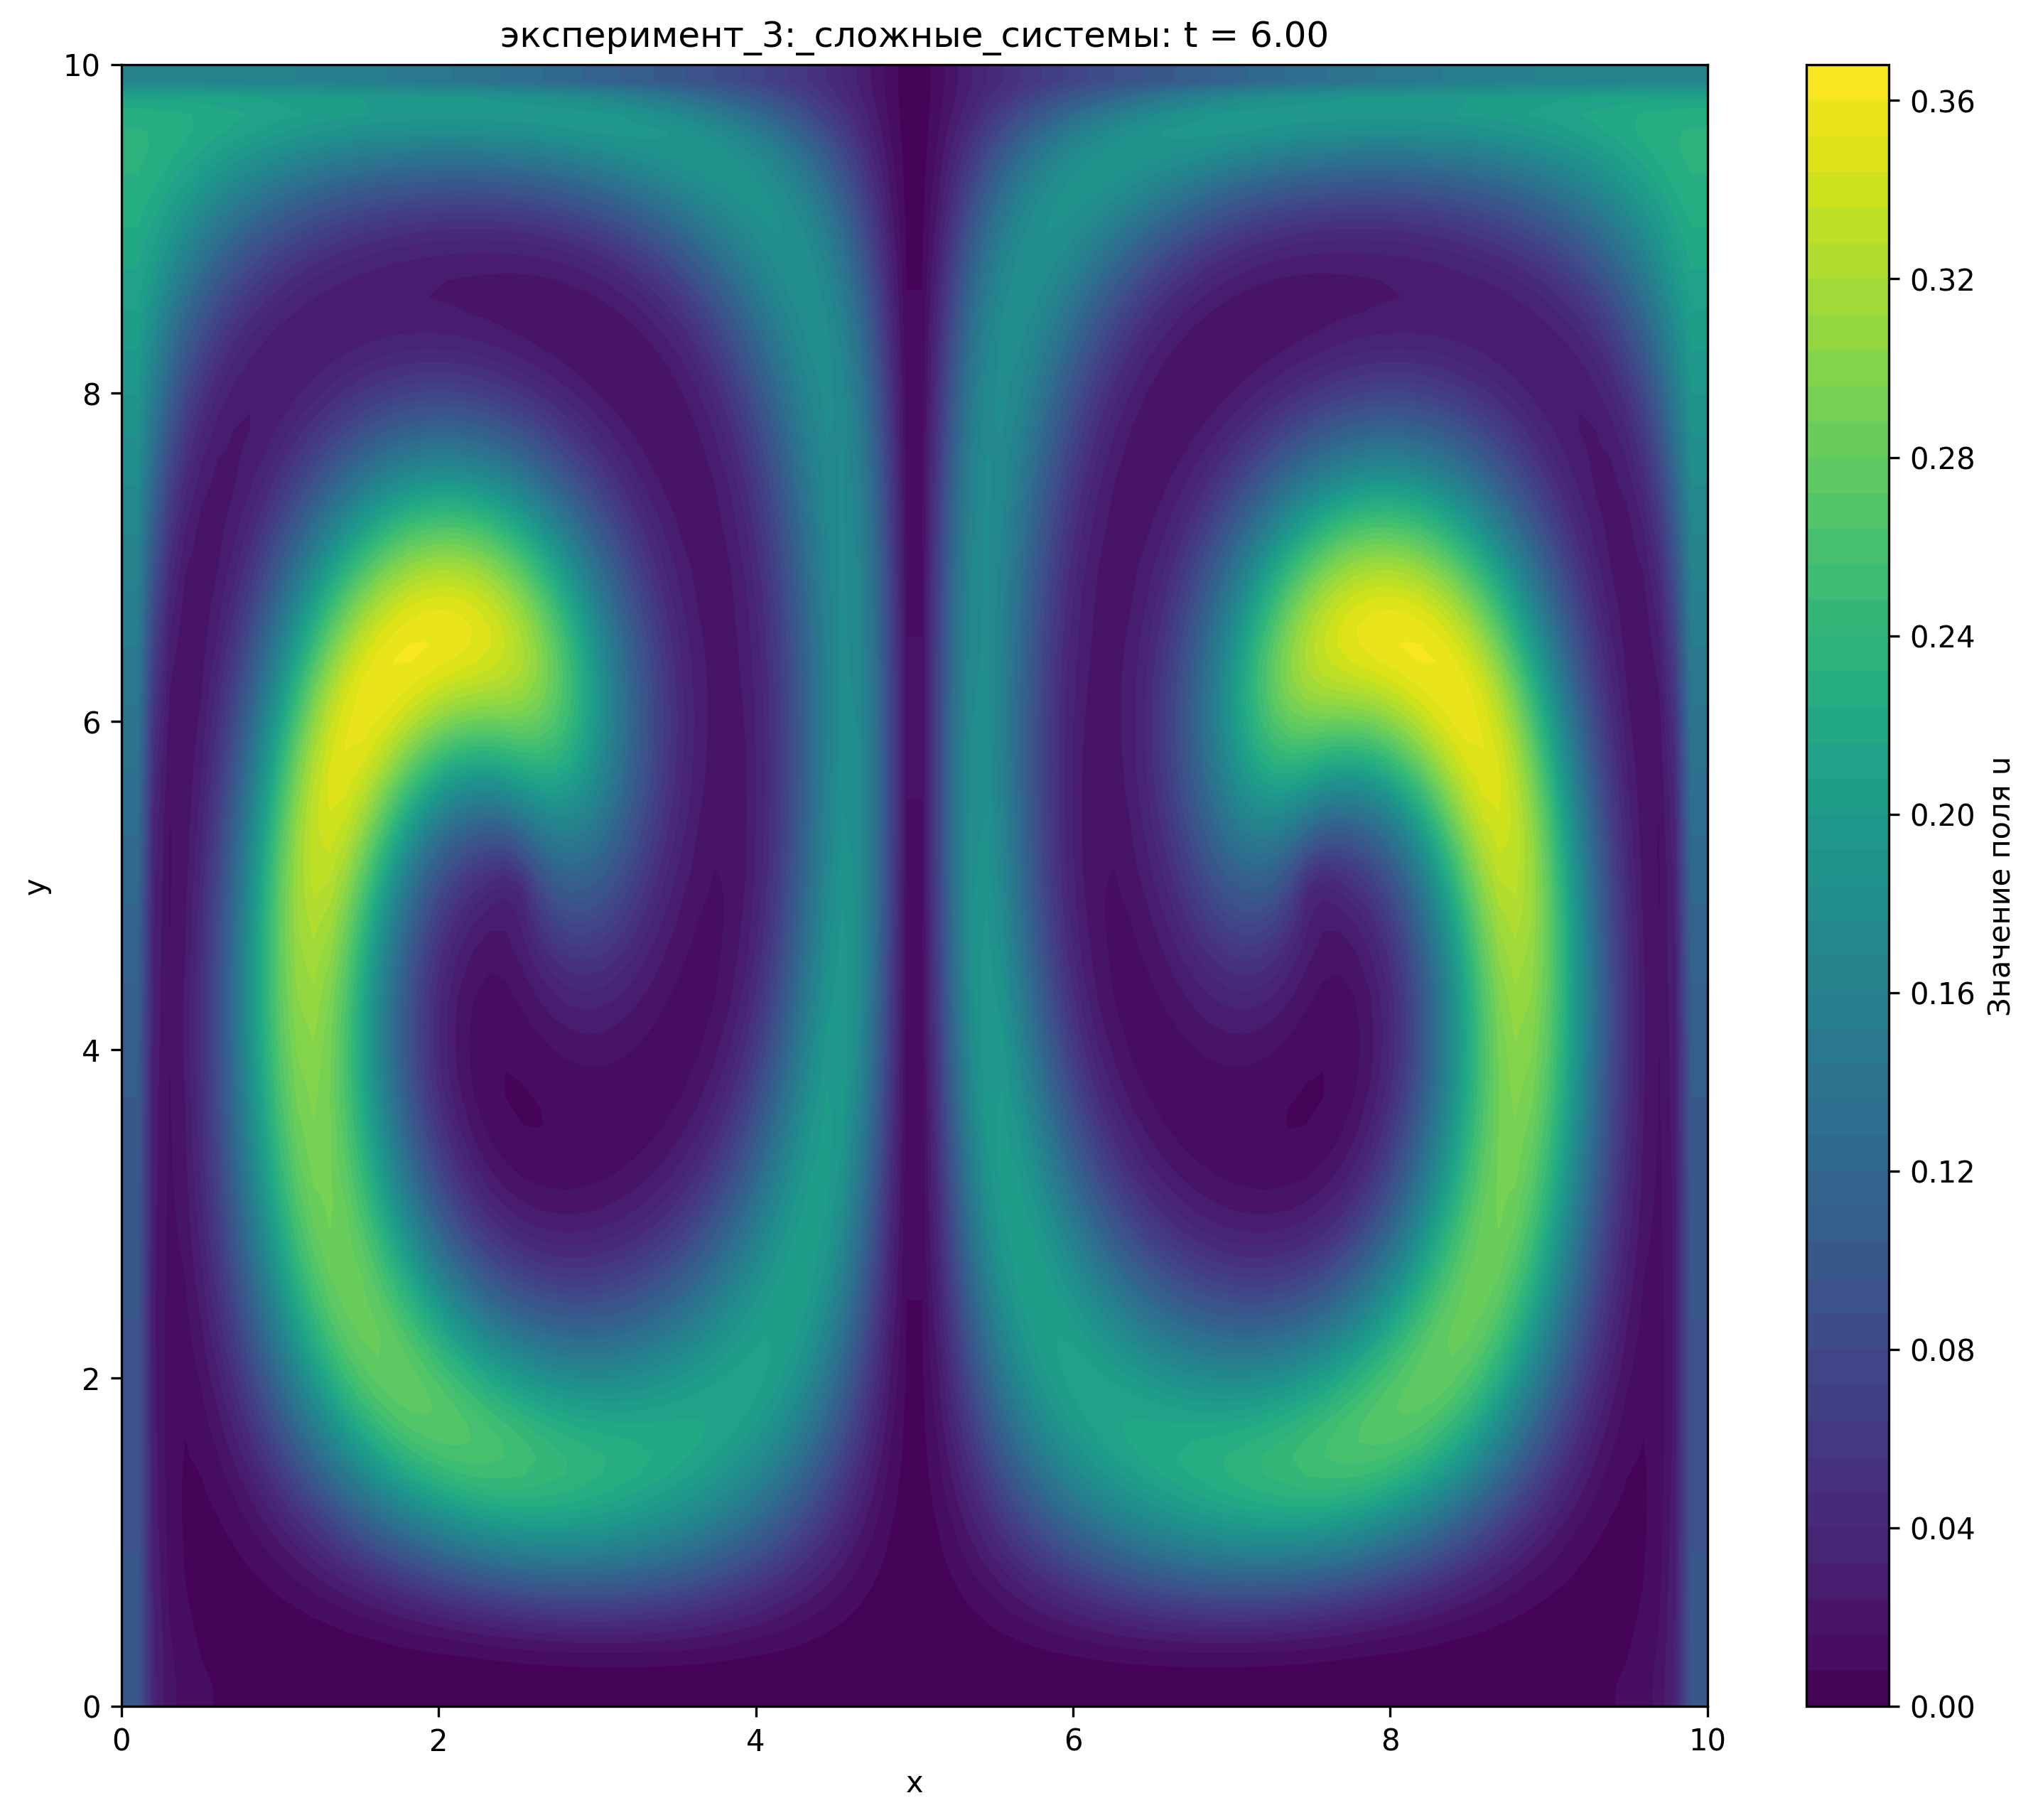
\includegraphics[width=0.6\textwidth]{imgs/эксперимент_3:_сложные_системы_t6.00.png}
	\caption{Скалярное поле в момент времени $t=6$ }
\end{figure}
\begin{figure}[h]
	\centering
	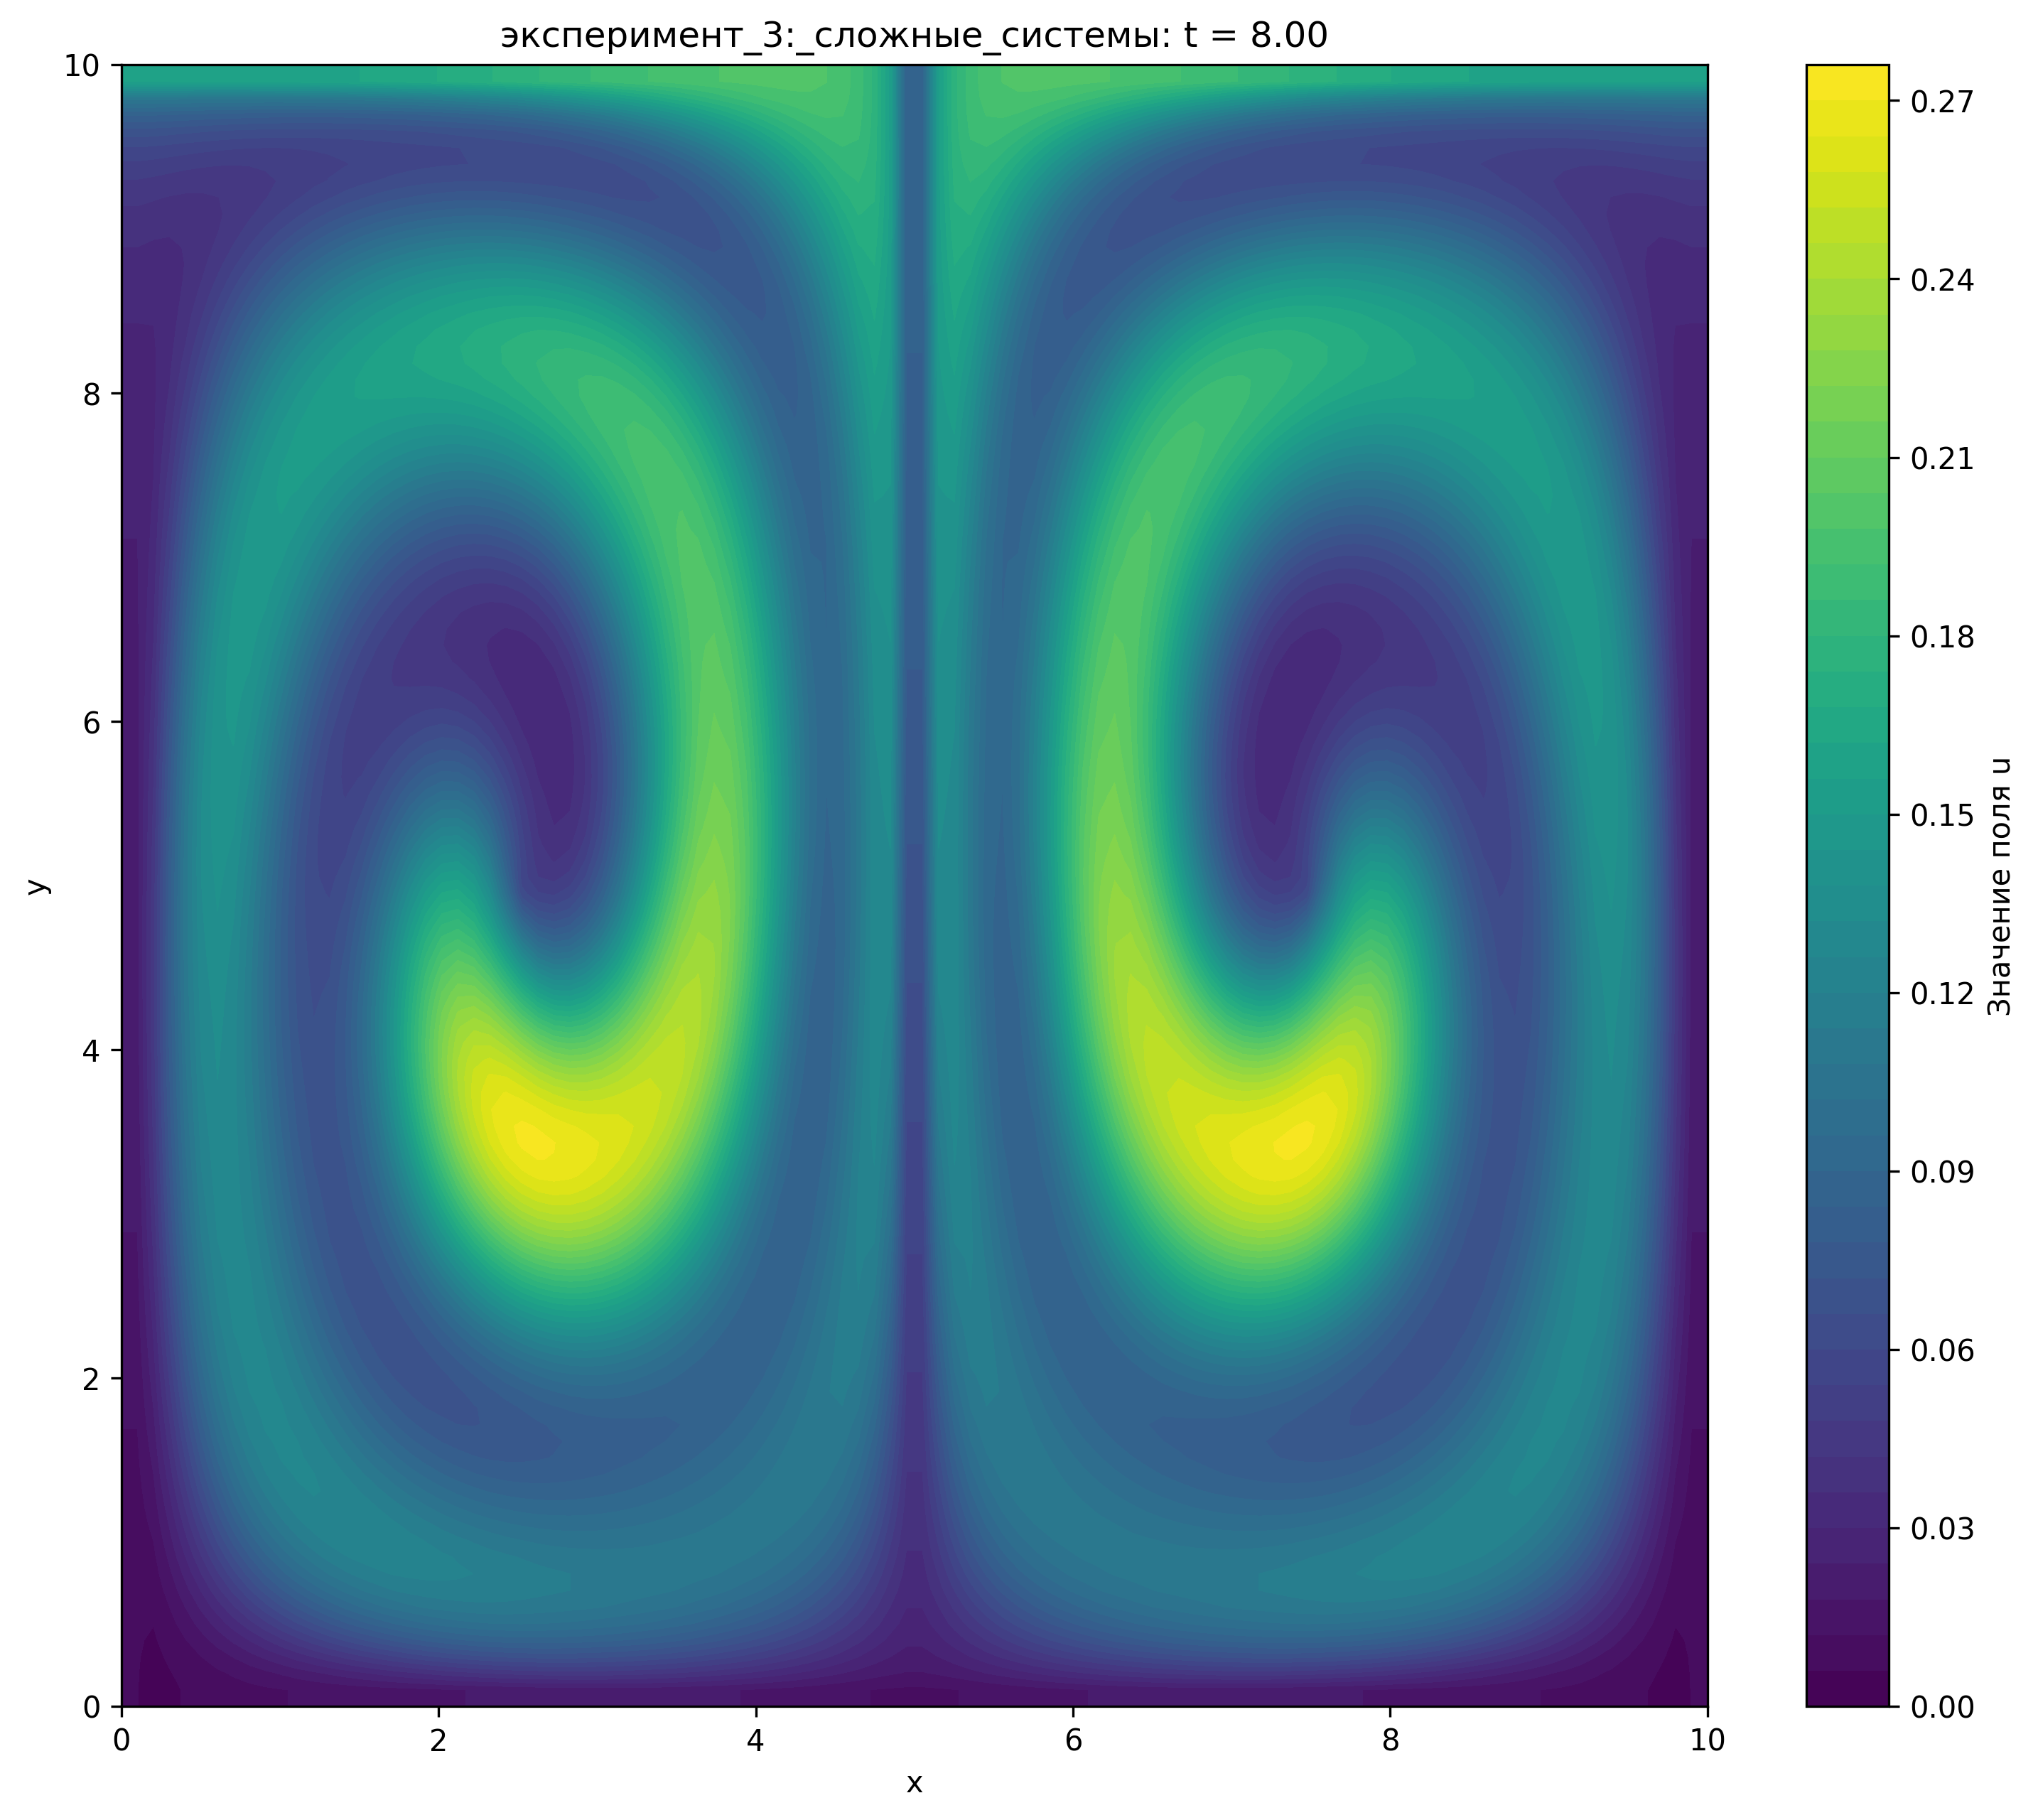
\includegraphics[width=0.6\textwidth]{imgs/эксперимент_3:_сложные_системы_t8.00.png}
	\caption{Скалярное поле в момент времени $t=8$}
\end{figure}